\documentclass{article}
\usepackage{graphicx}
%\graphicspath{{fig/}}
\usepackage{color}
\usepackage{epstopdf}
\usepackage{tabularx}
\usepackage{amssymb}
\usepackage{amsmath}
\usepackage{multirow}
\usepackage{array}
\usepackage{lineno}
\usepackage{booktabs}
\usepackage{threeparttable}
\usepackage{geometry}
\usepackage{setspace}
\usepackage{multirow}
\usepackage{caption}
\usepackage{hyperref}
\usepackage{authblk}
\usepackage{hyperref}
%
\newcommand*{\email}[1]{%
	\normalsize\href{mailto:#1}{#1}\par
}
\graphicspath{{./figs/}}
\geometry{left=2.5cm,right=2.5cm,top=2.5cm,bottom=2.5cm}
\setlength{\parskip}{0.5\baselineskip}
\linespread{1.25}
\usepackage{hyperref}
\title{Slow light waveguide design problem}
 \author{Fengwen~Wang}
 
 
\affil{Department of Mechanical Engineering, Technical University of Denmark, \\ Nils Koppels All{\'e}, Building 404, 2800 Kgs. Lyngby, Denmark\\ \email{fwan@mek.dtu.dk}}
 
\begin{document}
% \date{\today}
%\maketitle
This is an example of inverse design of slow light waveguides  based on supercell band structure calculations. For the $h_z$ polarization,  the band structure calculation is governed by
\begin{equation}\label{Equ:mast}
	\boldsymbol{\nabla} \cdot \left( \frac{1}{\varepsilon_r} \boldsymbol{\nabla} {h}\right)+ \left(\frac{\omega}{c}\right)^2 {h}=0  
\end{equation}
under the Floquet-Bloch wave boundary conditions as
\begin{equation}\label{Equ:mast1}
	{h}\left(x,a\right)=\exp\left(ika\right){h}\left(x,0\right) \qquad  {h}\left(0,y\right)={h}\left(b ,y\right). 
\end{equation} 

The discrete expression   obtained using the finite element method is stated as
\begin{equation}\label{Equ:FEM}
	\left( \mathbf{K}_k-{\omega}^2 \mathbf{M} \right)\mathbf{h}=0.
\end{equation}

  The considerd supercell, initial design and corresponding design domain are illustrated in the figure below.   

	\begin{figure}[!h]
	\centering
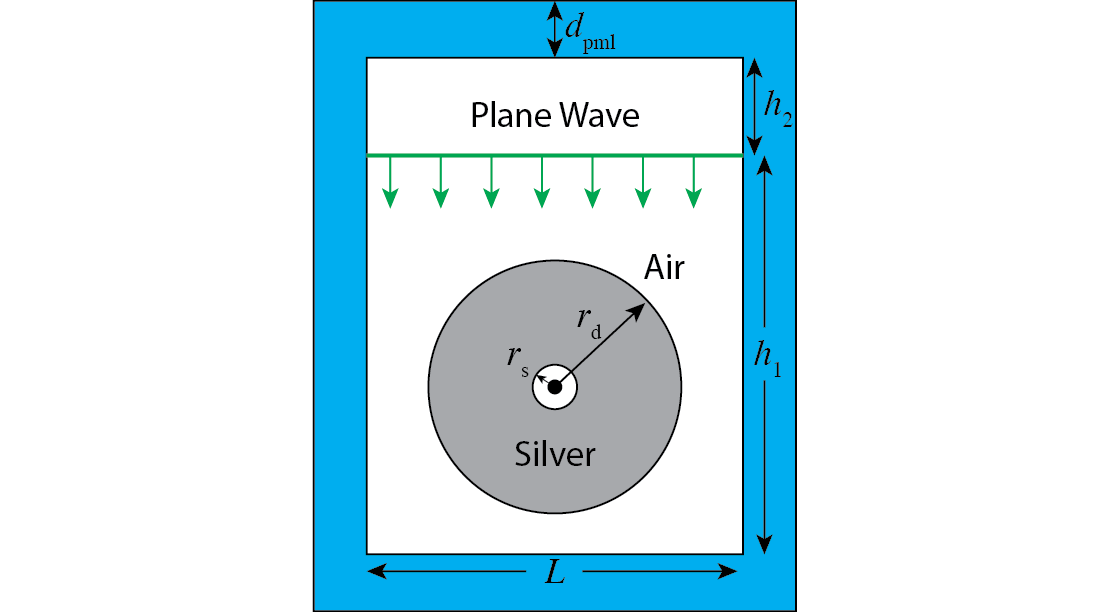
\includegraphics[width=0.95\textwidth]{Illustration.png} 
\end{figure}

The design problem is stated as
\begin{eqnarray}
	\min_{\rho_j} \ \ \max_{\eta}\ \ \max_{k_i} && f\left(\overline{\boldsymbol{\rho}}_\eta\right)= \left(\frac{c\left(k_i-k_{i-1}\right)}{{\omega}^{\eta}_n\left(k_{i-1}\right)-{\omega}^{\eta}_n\left(k_i\right)}-n^*_g\right)^2 \nonumber \\
	s.t.  && \left[ \mathbf{K}^{\eta}_k - \left({\omega}^{\eta} \right)^2 \mathbf{M}^{\eta} \right]\mathbf{h}^{\eta}=0  \nonumber \\
	&&  \max_{k_{ii}} \ \  {{\omega}^{\eta}_{n-1}\left(k_{ii}\right)} \  \leq \ a_1 \  \min_{k_i} \ \ {{\omega}^{\eta}_n\left(k_i\right)} \nonumber \\
	&&   {{\omega}^{\eta}_{n}\left(0\right)} \  \geq \ a_2 \ \max_{k_i} \ \ {{\omega}^{\eta}_n\left(k_i\right)}  \nonumber \\
	&& \min_{k_{ii}} \ \  {{\omega}^{\eta}_{n+1}\left(k_{ii}\right)} \  \geq \ a_2 \ \max_{k_i} \ \ {{\omega}^{\eta}_n\left(k_i\right)} \nonumber \\
	&&  f_v =\frac{\sum_{j} \overline{\rho}^{\eta}_j v_j}{\sum_{j} v_j }\leq 1 \nonumber \\
	&&   0\leq \rho_j \leq 1 \nonumber\\
	&& j=1,\ldots,N, \quad i=2,\ldots,m, \quad a_1 < 1, \quad a_2>1 . 
\end{eqnarray} 

The relevant parameters are defined below:
 
\begin{itemize}
	\item Discretization:
	
	 408x40 bilinear quadrilateral elements
	
\item 	Regularization: 

	density filter (filter radius: 1/8a) + projection
	\item Continuation scheme in the projection
	
	 For every $40$th iteration or if ( \{ $\Delta \rho< 1e-3$ or $\Delta f <1e-3$ \} and $\beta < 50$,   set $\beta=1.3 \beta$.  \\
  If $\Delta \rho < 1e-4$ or $\Delta f < 1e-4 $,  terminate. 

\item Interpolation of the relative permittivity of element $e$: 

$\frac{1}{\varepsilon^{\eta}_e} = \left(1- \overline{\rho}^{\eta}_e \right)\frac{1}{\varepsilon_{\rm{air}}} +\overline{\rho}^{\eta}_e  \frac{1}{\varepsilon_{\rm{Si}}}$ where $\varepsilon_{\rm{Si}}=(3.476)^2$.
\item 	Robust formulation: $ \eta \in [0.35, 0.5, 0.65]$.

\item $n^*_g=25$
\item Target $k$ points:
7  equidistant points $k \in [0.3875, 0.4625]2{\pi}/a$ 
\item $a_1=0.9$ and $a_2=1.1$
\end{itemize}
The blue print design  with $\eta=0.5$ obtained using the robust optimization formulation considering the parameters above and corresponding performance are shown in the figure below. 
 
	\begin{figure}[!h]
	\def\svgwidth{1\textwidth}
	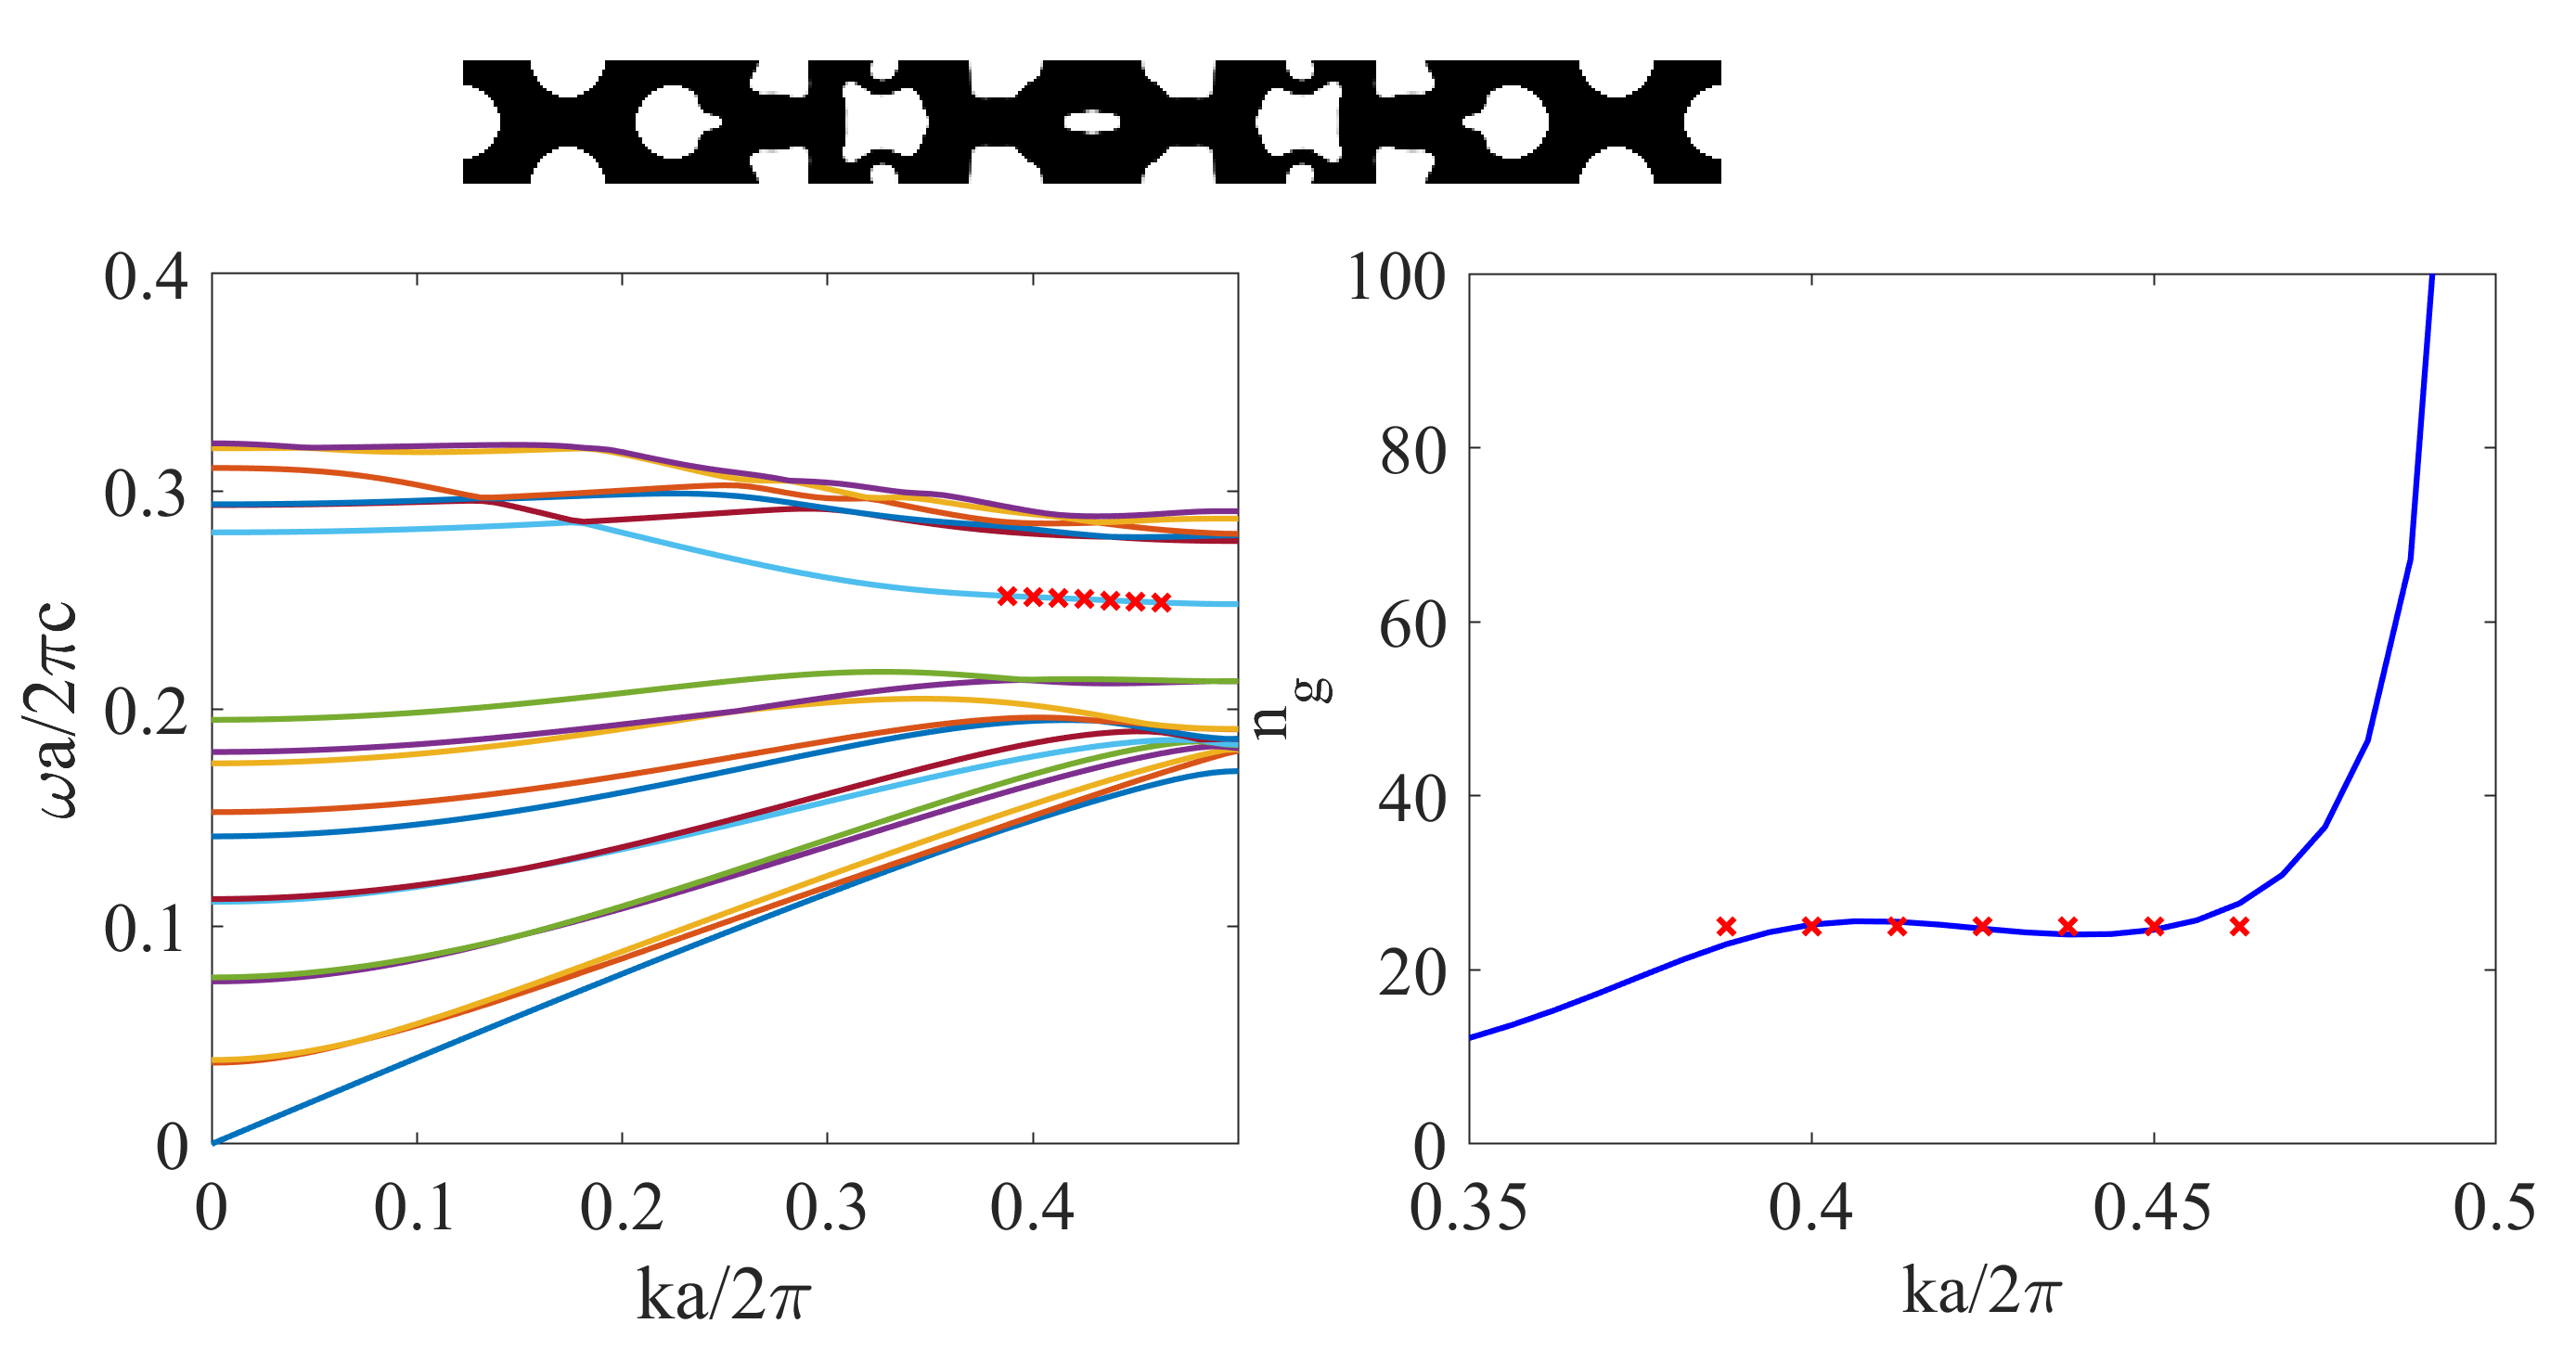
\includegraphics[width=\textwidth]{Resp_Dnum_2_FF.png} 
\end{figure}
%\end{linenumbers}
\end{document}














